% vim: set textwidth=78 autoindent:

\subsection{Georeferenzier Plugin}\index{Plugins!Georeferenzierer}

% when the revision of a section has been finalized, 
% comment out the following line:
%\updatedisclaimer

Das Plugin \toolbtntwo{georeferencer}{Georeferenzierer} erlaubt die
Erstellung von World files f�r Rasterkarten. Damit das Plugin die World file
Parameter berechnen kann, w�hlen sie auf einer Rasterkarte Punkte aus und
ordnen diesen Punkten die entsprechenden Koordinaten zu. Das Ergebnis der
Georeferenzierung wird umso genauer, je mehr Koordinaten Sie dem Plugin zur
Verf�gung stellen.

Als Beispiel hierf�r soll ein World file f�r eine topografische Karte aus der
Gegend S�d-Dakotas erstellt werden, welche zu dem GRASS Spearfish-Datensatz
passt. Diese Karte kann sp�ter zusammen mit den erstellten Daten in
der GRASS spearfish60 Location dargestellt werden. Die topopgrafische Karte
steht unter folgender Adresse zum Download bereit.
\url{http://grass.osgeo.org/sampledata/spearfish\_toposheet.tar.gz}

Als erstes laden Sie bitte die topopgrafische Karte herunter und entpacken
diese mit dem tar-Befehl.

\begin{verbatim}
wget http://grass.osgeo.org/sampledata/spearfish_toposheet.tar.gz
tar xvzf spearfish_toposheet.tar.gz
cd spearfish_toposheet
\end{verbatim}

Als n�chstes starten Sie QGIS, laden dort das Georeferenzierungs-Plugin und
w�hlen dann die spearfish\_topo24.tif aus.

\begin{figure}[ht]
\begin{center}
\caption{Ausw�hlen des zu georeferenzierenden Bildes \nixcaption}\label{fig:select_image}\smallskip
  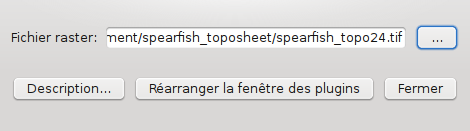
\includegraphics[clip=true, width=10cm]{select_image}
\end{center}
\end{figure}

Dann klicken Sie auf den Knopf \button{Fenster anordnen}, um das ausgew�hlte
Bild im Georeferenzierer zu �ffnen und auf dem Desktop gemeinsam mit dem QGIS
Kartenfenster optimal anzuordnen (siehe Abbildung~\ref{fig:georefplugin}).

\begin{figure}[ht]
\begin{center}
  \caption{Das Plugin- und Kartenfenster optimal anordnen \nixcaption}\label{fig:georefplugin}\smallskip
  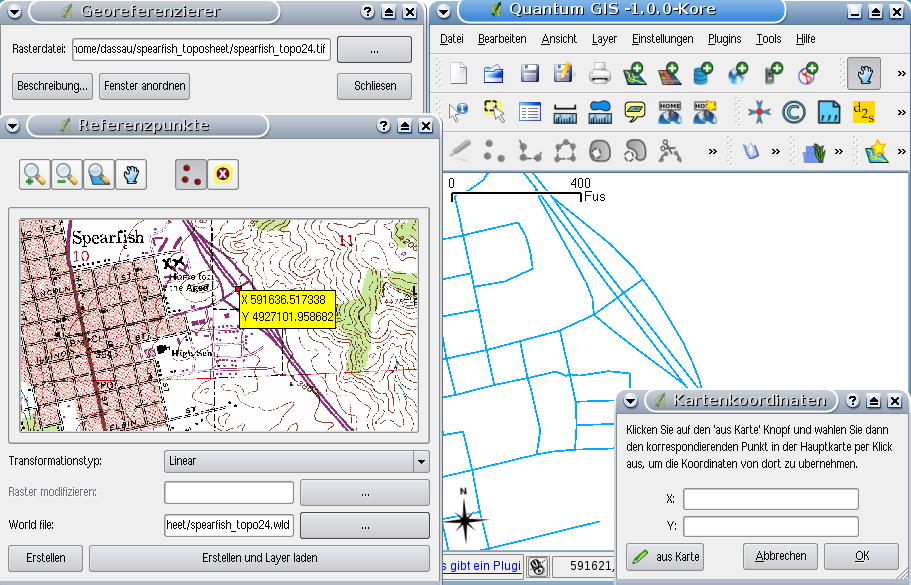
\includegraphics[clip=true,width=0.9\textwidth]{georefplugin}
\end{center}
\end{figure}

Mit dem Knopf \button{Addiere Punkt} k�nnen Sie nun damit beginnen dem
Rasterbild Punkte und die dazugeh�rigen Koordinaten hinzuzuf�gen (siehe
Abbildung~\ref{fig:choose_points}). Aus diesen Punktkoordinaten errechnet das
Plugin die entsprechenden World file Parameter. Je mehr Koordinaten Sie dem
Plugin zur Berechnung zur Verf�gung stellen, desto genauer wird das Ergebnis.
F�r die Angabe der n�tigen Punktkoordinaten stehen Ihnen zwei
unterschiedliche Vorgehensweisen zur Verf�gung.

\begin{enumerate}
\item Sie klicken auf einen Punkt in der Rasterkarte und geben die X- und
Y-Koordinaten ein.
\item Sie klicken auf einen Punkt in der Rasterkarte und w�hlen den Knopf
\button{aus Karte} um die X- und Y-Koordinaten mit Hilfe einer
georeferenzierten, in QGIS geladenen Karte hinzuzuf�gen.
\end{enumerate}

\begin{figure}[ht]
\begin{center}
  \caption{Punkte zu einem Rasterbild hinzuf�gen \nixcaption}\label{fig:choose_points}\smallskip
  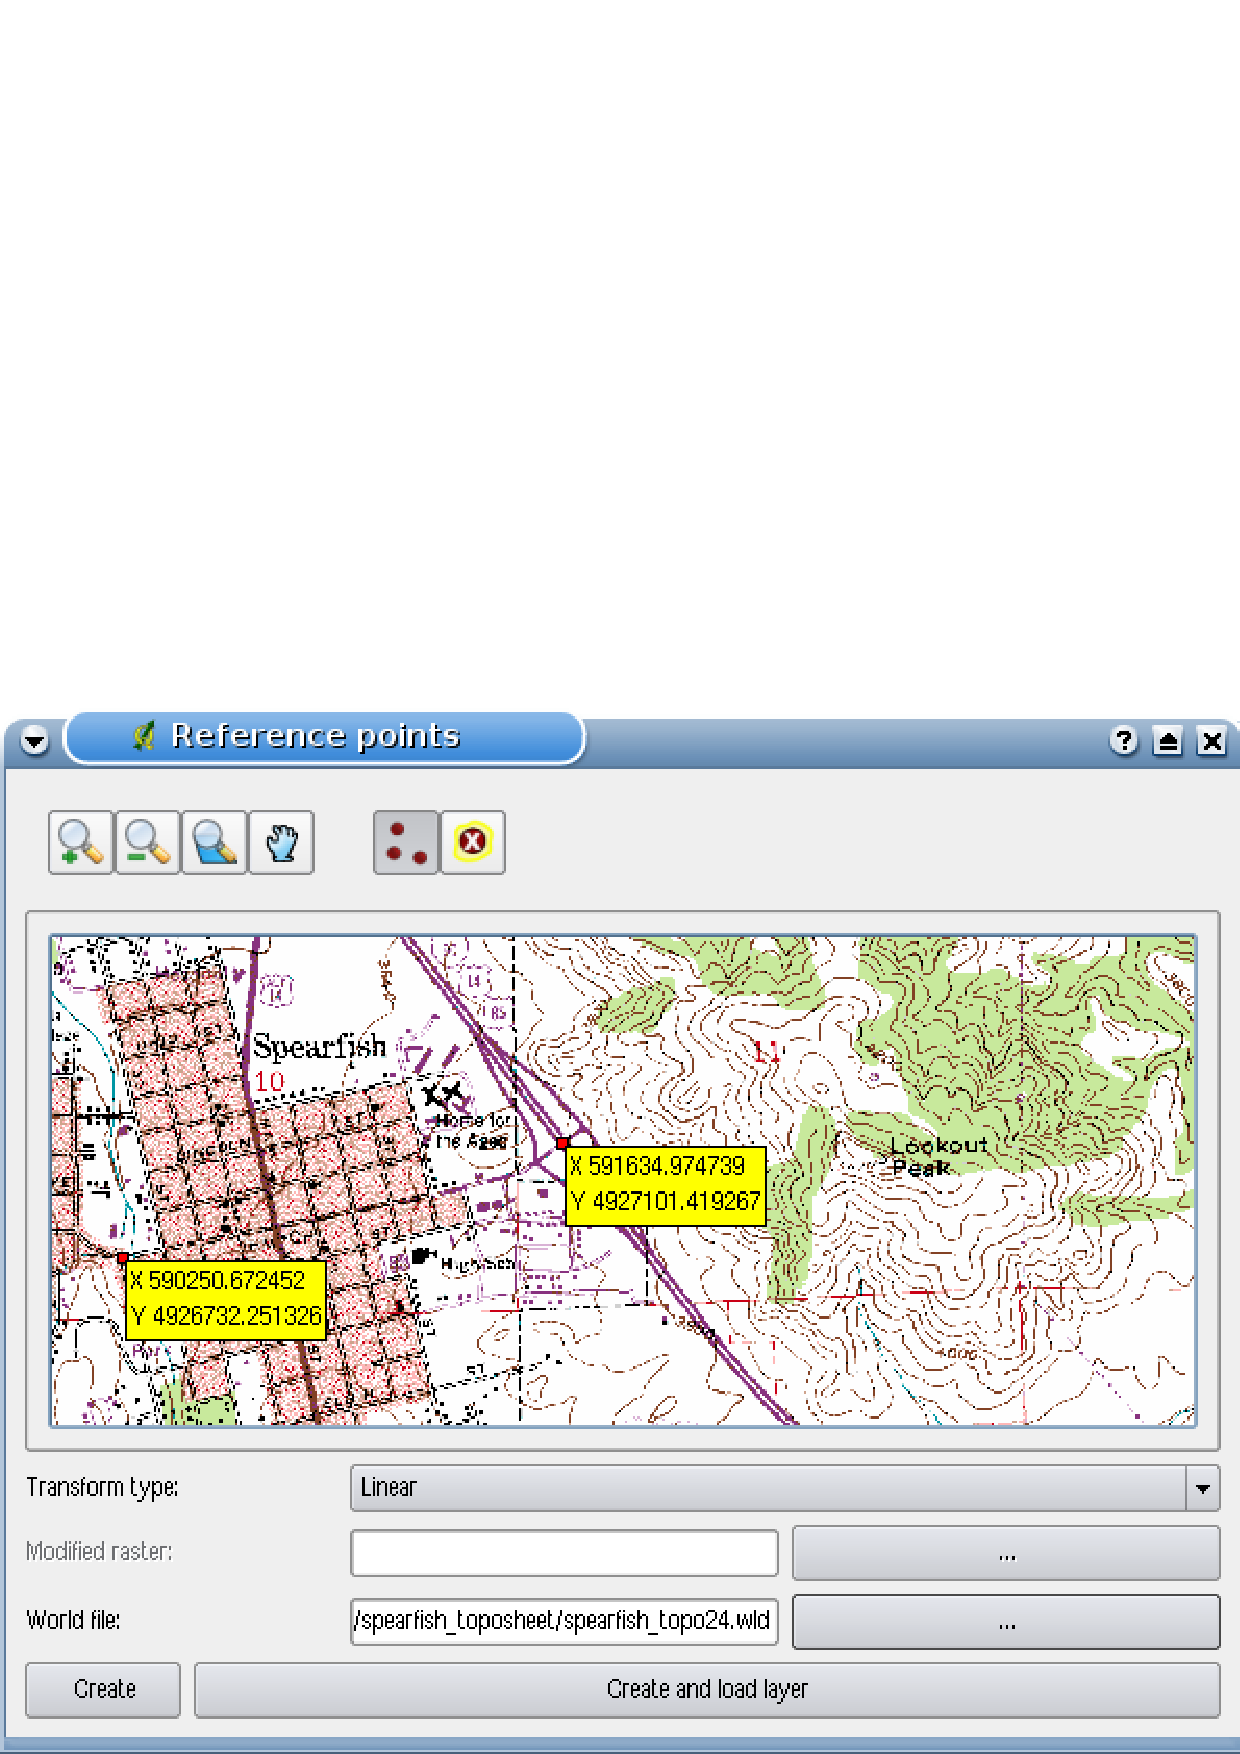
\includegraphics[clip=true,width=0.9\textwidth]{choose_points}
\end{center}
\end{figure}

In unserem Beispiel nutzen wir die zweite Option und geben die Koordinaten
der ausgew�hlten Punkte mit Hilfe des Vektorlayers \filename{roads} aus der
\usertext{spearfish60} Location ein. Diese Daten stehen unter folgender
Adresse zum Download bereit: \\
\url{http://grass.osgeo.org/sampledata/spearfish\_grass60data-0.3.tar.gz}

F�r den Fall, dass Sie nicht wissen, wie Sie die spearfish60 Location in QGIS
integrieren und mit Hilfe des GRASS Plugins verwenden k�nnen, finden Sie im
Abschnitt~\ref{sec:grass} weitere Informationen. 

Wie Sie in Abbildung~\ref{fig:choose_points} sehen k�nnen, stellt Ihnen der
Georeferenzierdialog Kn�pfe zum Vergr��ern/Verkleinern, zum Verschieben,
sowie zum Hinzuf�gen und L�schen von Punkten in der Karte zur Verf�gung. 

Nachdem Sie dem Bild eine ausreichende Anzahl an Punkten gesetzt haben,
gilt es nun, f�r den Georeferenzierungs-Vorgang die gew�nschte
Koordinaten-Transformationsmethode auszuw�hlen und die daraus errechneten
world-file Daten zusammen mit dem Tiff zu speichern. In unserem Beispiel
entscheiden wir uns f�r den \selectstring{Transformationstyp}{Linear}, wobei
der \selectstring{Transformationstyp}{Helmert} wahrscheinlich auch ein
ausreichendes Ergebnis liefern w�rde.

\begin{Tip}\caption{\textsc{Wahl des Transformationstyps}}
\qgistip{Die lineare (affine) Koordinaten-Transformationsmethode ist eine
Transformation erster Ordnung und wird zur Skalierung, Umwandlung und
Drehung von geometrisch fehlerfreien Bildern verwendet. Im Falle der
Helmert-Transformation werden einem Bild - wie beim geokodieren - einfach
Koordinaten-Informationen hinzugef�gt. Ist ihr Bild verzerrt, so ben�tigen
Sie Programme, die eine polynome Transformation zweiter
und dritter Ordnung erm�glichen, wie z.B. GRASS GIS.
}
\end{Tip} 

Die von uns gesetzten Punkte werden zusammen mit dem Rasterbild in der
Datei \filename{spearfish\_topo24.tif.points} gespeichert. Dies erlaubt uns,
bei Bedarf das Georeferenzier Plugin wieder zu �ffnen und neue Punkte
hinzuzuf�gen oder bestehende Punkte zu l�schen, um dadurch das Ergebnis zu
verbessern. Die Datei \filename{spearfish\_topo24.tif.points} zeigt
beispielsweise folgende Punkte an:  

\begin{verbatim}
mapX    		mapY    		pixelX  pixelY
591630.196867999969982  4927104.309682800434530 591647  4.9271e+06
608453.589164100005291  4924878.995150799863040 608458  4.92487e+06
602554.903929700027220  4915579.220743400044739 602549  4.91556e+06
591511.138448899961077  4915952.302661700174212 591563  4.91593e+06
602649.526155399973504  4919088.353569299913943 602618  4.91907e+06
\end{verbatim} 

Um das Rasterbild zu georeferenzieren, wurden hier 5 Koordinatenpunkte
verwendet. Um m�glichst genaue Resultate zu erhalten, ist es wichtig, die
verschiedenen Punkte gleichm��ig innerhalb des Bildes zu verteilen. Zum Abschluss
�berpr�fen wir das Ergebnis, laden die neue georeferenzierte Karte
\filename{spearfish\_topo24.tif} in QGIS und �berlagern diese mit dem
Vektorlayer \filename{roads} aus der spearfish60 Location.  

\begin{figure}[ht]
\begin{center}
  \caption{Georeferenzierte Karte mit �berlagerten Strassen der spearfish60
Location \nixcaption}\label{fig:result_map}\smallskip
  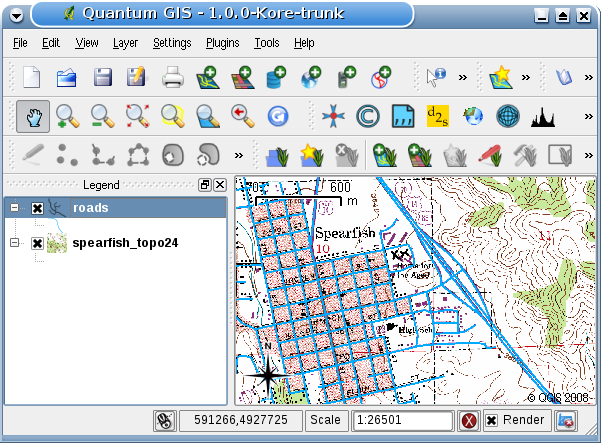
\includegraphics[clip=true,width=0.85\textwidth]{result_map}
\end{center}
\end{figure}

